\specialchapter{PLATE X. IRREDUCIBLE SYSTEMS OF RANK 2}

\pandocbounded{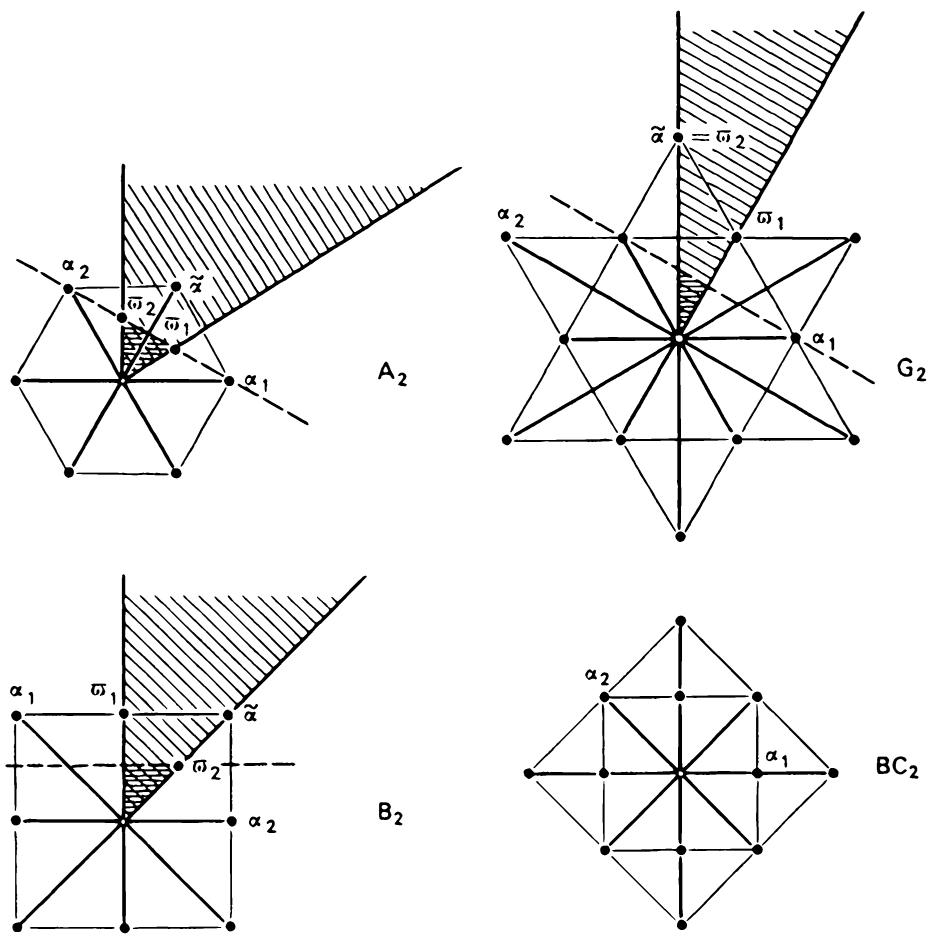
\includegraphics[keepaspectratio]{images/part002_e5dc67b9.jpg}}\\
The first three diagrams above represent the root systems R of type \(A_{2}\) . \(B_{2}\) and \(G_{2}\) . The shaded region represents the chamber C corresponding to the basis \((\alpha_{1},\alpha_{2})\) . The line \((x|\beta)=1\) , where \(\beta\) denotes the highest root of the

inverse system \(R^{-}\) , is shown dotted, and the doubly shaded region represents the alcove of \(R^{-}\) with vertex 0 contained in C.

The last diagram represents the unique irreducible non-reduced root system of rank 2.
% semantic-fragments: legacy-input-seam
\relax{}
